% Chapter 5

\chapter{Experimental results} % Main chapter title

\label{Chapter5} % For referencing the chapter elsewhere, use \ref{Chapter5} 

%----------------------------------------------------------------------------------------
\section{Introduction}
In the previous chapters we described how the DeepMiRNA's architecture is based on two main functional blocks: on one side there is the NN, whose purpose is that of analyzing the selected candidate target sites, while on the other there are the CSSM used during the target prediction step and the a-posteriori filter that tries to refine the network prediction. 

To assess these two aspects, we first evaluated the outputs of the NN training process through cross validation and then investigated performance using the different candidate site selection methods outlined in chapter \ref{Chapter3}. These comprised the novel (non-canonical) models implemented for this thesis: CSS-6.10 and CSS-7.10. Finally, we tested DeepMiRNA’s performance by comparing it against TargetScan\cite{targetscan}, mirDB\cite{mirdb} and miRAW\cite{miraw}, which represent the most commonly used target site predictors based on citations.

\section{Neural Netework evaluation}
The best performing feed-forward neural network was trained using the whole training set with this parameters:

\begin{itemize}
	\item dropout rate = 0.7
	\item optimizer = Adam as described in chapter \ref{Chapter4}
	\item loss function = binary cross entropy
	\item batch size = 128
	\item number of epochs = 15
\end{itemize}

The above parameters where computed using a validation set composed of about 10000 examples (20\% of the training set).

Once the best model has been selected, we built a fresh network using the best parameters and we trained it holding out the 25\% of the training data for the purpose of testing its performance. This validation presented very good results in terms of predicting both positive and negative sites, with all evaluated metrics resulting in scores well above 0.9 (see figure\ref{fig:network_evaluation}).

\begin{figure}[hbt!]
	\centering
	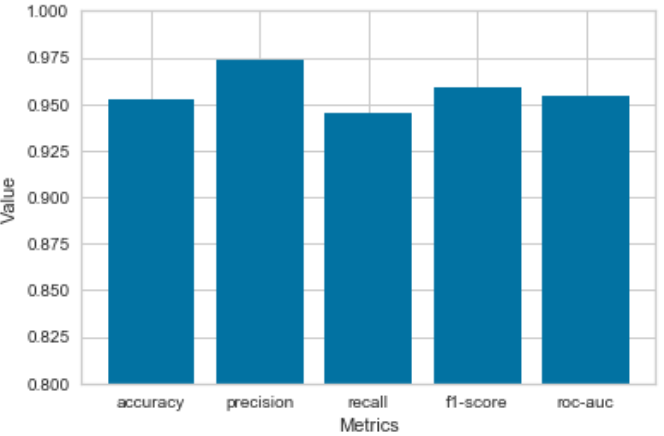
\includegraphics[width=\textwidth]{Figures/network_evaluation}
	\caption{\textbf{Network performance metrics.} To this purpose we trained the network with best parameters using 75\% of the training data. The remaining 25\% has been used as test set. As shown above all metrics are close to 0.95.}
	\label{fig:network_evaluation}
\end{figure}

\section{The role of the candidate site selection method}
To investigate the impact of the site selection method, we compared the performances of the three different CSSM described in chapter\ref{Chapter3}. 

Figure \ref{fig:cssm} summaries the obtained results: all methods reach accuracies between 0.76 and 0.8, these values are computed considering the imbalance of the test set, that is they are calculated as the average of the accuracies on positive and negative samples. CSS-6.0:10 seems to achieve slightly better performances for every metric compared to the other two methods. This is the less conservative approach and represents the best trade-off between the higher quantity of false positives generated by the CSSM and the increased rate of false negatives due to the filtering stage. The F1-score is the harmonic average between precision and recall and shows how well both classes are classified by a particular CSSM. The values obtained are very similar to the accuracies and indicate an ability to effectively predict both negative and positive targets especially for CSS-6.0:10 and CSS-7.0:10.

\begin{figure}[hbt!]
	\centering
	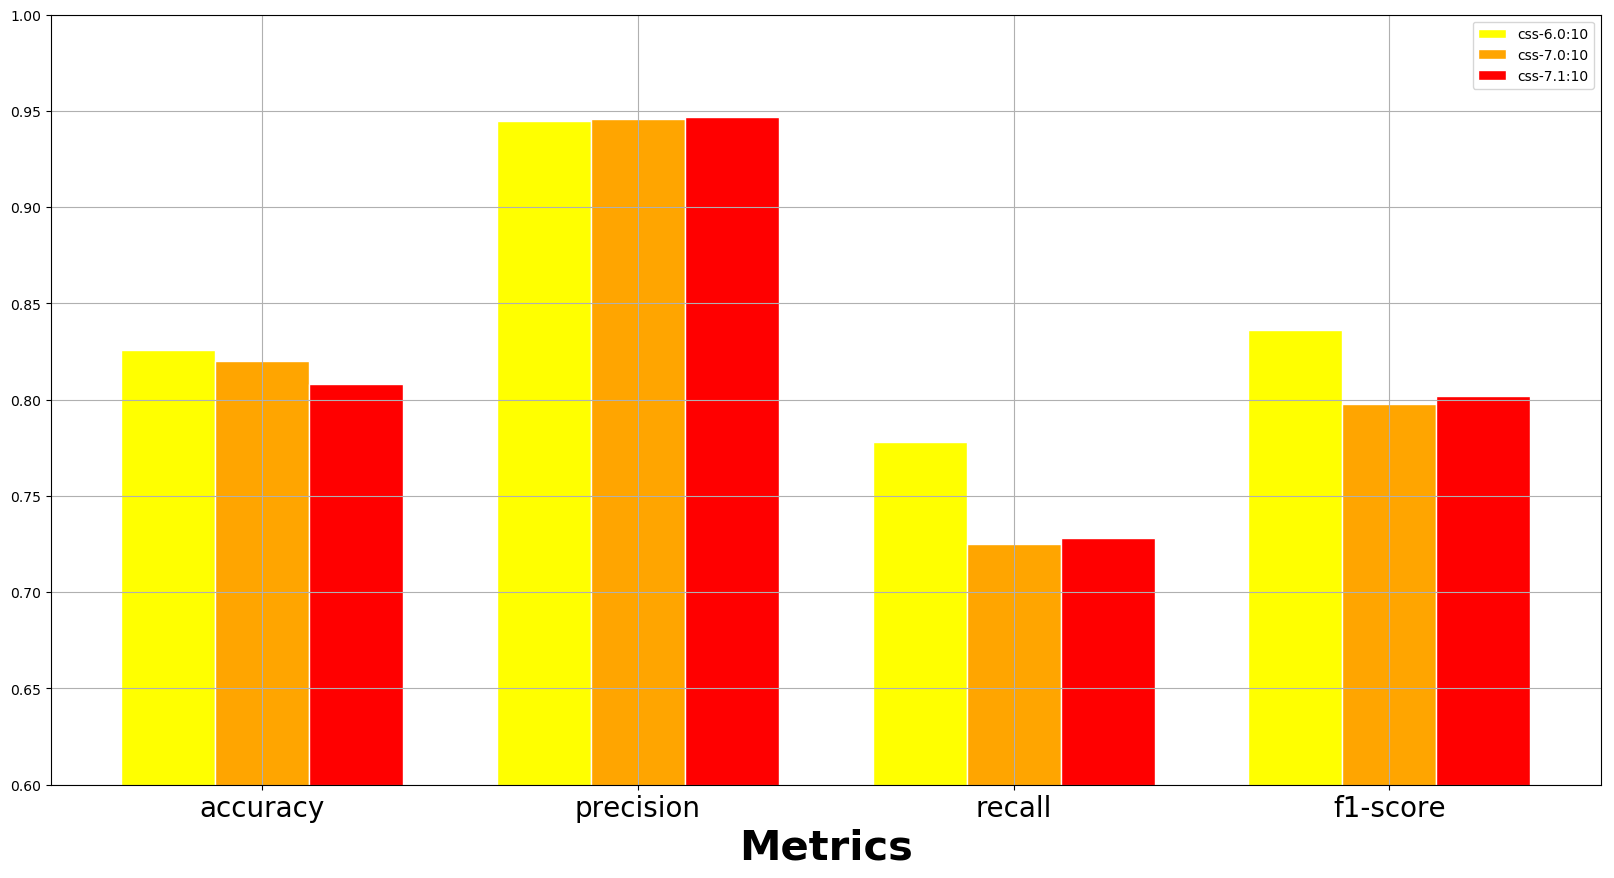
\includegraphics[width=\textwidth]{Figures/cssm_evaluation}
	\caption{\textbf{Evaluation of DeepMiRNA different candidate site selection methods.} Results are evaluated in terms of balanced accuracy, precision, recall and f1-score. The best result was achieved using CSS-6.0:10.}
	\label{fig:cssm}
\end{figure}

\section{The importance of site accessibility filtering}
In order to measure the effect of site accessibility on miRNA target prediction, we tested the best performing pipeline configuration without filtering the network output. While this considerably reduce the computational cost of the whole process, DeepMiRNA becomes more biased towards the prediction of positive sites which resulted in high recall but low precision. The obtained results are compared in Table \ref{tab:sa_filter}.     

\begin{table}
	\caption{\textbf{Comparison results with or without the a-posteriori filter}}
	\label{tab:sa_filter}
	\centering
	\begin{tabular}{| c | c | c | c | c | c | c | c |} \hline
		\multicolumn{2}{|c|}{Accuracies} & \multicolumn{2}{c|}{Precision} & \multicolumn{2}{c|}{Recall} & \multicolumn{2}{c|}{F1-score} \\ \hline 
		NF & WF & NF & WF & NF & WF & NF & WF \\ \hline
		
		
	\end{tabular}
\end{table}
